\documentclass[10pt]{article}
\usepackage{trymtex}
\usepackage{multicol}
\usepackage{enumitem}
\usepackage{booktabs}
\setlist{noitemsep, topsep=0pt, parsep=0pt, partopsep=0pt}
% bright red
\definecolor{formulacolor}{RGB}{255, 69, 0}
\pagestyle{empty}
\makeatletter
% section formatting (minimal spacing)
\renewcommand{\section}{\@startsection{section}{1}{0mm}
  {-0.1ex}%
  {0.1ex}%
  {\normalfont\normalsize\bfseries\color{thm-color}}} 
\renewcommand{\subsection}{\@startsection{subsection}{2}{0mm}
  {-0.1ex}%
  {0.1ex}%
  {\normalfont\small\bfseries\color{rem-color}}}
\renewcommand{\subsubsection}{\@startsection{subsubsection}{3}{0mm}
  {-0.1ex}%
  {0.1ex}%
  {\normalfont\footnotesize\bfseries\color{cor-color}}}
\makeatother

\setcounter{secnumdepth}{0}
\setlength{\parindent}{0pt}
\setlength{\parskip}{0.5em}

\usepackage{titlesec}
\AtBeginDocument{
  \setlength{\abovedisplayskip}{3pt}
  \setlength{\belowdisplayskip}{3pt}
  \setlength{\abovedisplayshortskip}{3pt}
  \setlength{\belowdisplayshortskip}{3pt}
}

\pgfplotsset{compat=newest}
\geometry{landscape, margin=0.25cm, nohead, nofoot}
\setlength{\columnsep}{0.5cm}
\setlength{\parindent}{0pt}
\setlength{\parskip}{0.5em}
\renewcommand{\baselinestretch}{1.0}
\renewcommand{\thefootnote}{\fnsymbol{footnote}}
\newcommand{\noin}{\noindent}    
\newcommand{\logit}{\textrm{logit}} 
\newcommand{\var}{\mathrm{Var}}
\newcommand{\Var}{\mathrm{Var}}
\newcommand{\Cov}{\mathrm{Cov}} 
\newcommand{\corr}{\textrm{Corr}}
\newcommand{\Corr}{\mathrm{Corr}}
\renewcommand{\N}{\mathcal{N}}
\renewcommand{\E}{\mathrm{E}}
\newcommand{\Bern}{\textrm{Bern}}
\newcommand{\Bin}{\textrm{Bin}}
\newcommand{\Beta}{\textrm{Beta}}
\newcommand{\Gam}{\textrm{Gamma}}
\newcommand{\Expo}{\textrm{Expo}}
\newcommand{\Pois}{\textrm{Pois}}
\newcommand{\Unif}{\textrm{Unif}}
\newcommand{\Geom}{\textrm{Geom}}
\newcommand{\NBin}{\textrm{NBin}}
\newcommand{\Hypergeometric}{\textrm{HGeom}}
\newcommand{\HGeom}{\textrm{HGeom}}
\newcommand{\Mult}{\textrm{Mult}}
\newcommand{\SE}{\textrm{SE}}
\newcommand{\rank}{\textrm{rank}}
\newcommand{\vect}[1]{\symbf{#1}} % bold vectors
\newcommand{\mat}[1]{\symbf{#1}}  % bold matrices

 \newcommand\independent{\protect\mathpalette{\protect\independenT}{\perp}}
    \def\independenT#1#2{\mathrel{\setbox0\hbox{\( #1#2 \)}%
    \copy0\kern-\wd0\mkern4mu\box0}}
  
\usepackage{pgfplots}
\pgfplotsset{compat=newest}
\pgfmathdeclarefunction{gamma}{1}{%
  \pgfmathparse{%
    (#1 == 0.5) * 1.77245385090551602729 + % sqrt(pi)
    (#1 == 1.0) * 1.0 +
    (#1 == 1.5) * 0.88622692545275801364 + % sqrt(pi)/2
    (#1 == 2.0) * 1.0 +
    (#1 == 2.5) * 1.32934038817913702282 + % 3*sqrt(pi)/4
    (#1 == 3.0) * 2.0 +
    (#1 == 3.5) * 3.32335097044784255705 % 15*sqrt(pi)/8
  }%
}
\begin{document}
\scriptsize
\begin{multicols}{3}
  \section{Probability \& Distributions}
  \section{Multivariate Distributions \& Moments}
  \textup{if} \( X_{1},\dots,X_{n} \) are \textbf{i.i.d.} with \textit{CDF} \( F(\vect{x}) \) \textup{then}:
  \begin{align*}
    F_{X_{\min}}(\vect{x}) & = 1-[1-F(\vect{x})]^{n} \\
    F_{X_{\max}}(\vect{x}) & = [F(\vect{x})]^{n}
  \end{align*}
  For random vector \( \vect{X}\in\mathbb{R}^p \), covariance matrix:
  \[\Sigma = \mathrm{Cov}(\vect{X})=\E[(\vect{X}-\E[\vect{X}])(\vect{X}-\E[\vect{X}])^T] \in \mathbb{R}^{p\times p}\]
  \textit{Properties:}
  \begin{itemize}[left=0pt,labelsep=1pt]
    \item if \( a \) is constant vector then: \( \var(a^T \vect{X})=a^T\Sigma\,a \)
    \item if \( \vect{X} \independent \vect{Y} \) then \( \var(\vect{X}+\vect{Y})=\var(\vect{X})+\var(\vect{Y}) \)
  \end{itemize}
  \textit{Covariance:}
  \begin{align*}
    \var(\vect{X})                   & = \mathrm{diag}(\Sigma) = \mathrm{E}[(\vect{X}-\vect{\mu})(\vect{X}-\vect{\mu})^T]                                                                                                               \\
    \mathrm{Cov}(\vect{X},\vect{Y})  & = \mathrm{E}[(\vect{X}-\vect{\mu})(\vect{Y}-\vect{\nu})^T] = \mathrm{E}[\vect{X}\vect{Y}^T] - \mathrm{E}[\vect{X}]\mathrm{E}[\vect{Y}] = \mathrm{E}[\vect{X}\vect{Y}^T] - \vect{\mu}\vect{\nu}^T \\
    \mathrm{Corr}(\vect{X},\vect{Y}) & = \frac{\mathrm{Cov}(\vect{X},\vect{Y})}{\sqrt{\mathrm{Var}(\vect{X})\mathrm{Var}(\vect{Y})}} = \frac{\Cov(X_i,X_j)}{\sqrt{\var(X_i)\var(X_j)}}
  \end{align*}
  \section{Multivariate Normal (MVN):}
  \( \vect{X}\sim N_p(\vect{\mu},\Sigma) \) means \( \vect{X} \) has density
  \[f_X(\mathbf{\vect{x}}) = \frac{1}{(2\pi)^{p/2}|\Sigma|^{1/2}}\exp\{-\frac{1}{2}(\vect{x}-\vect{\mu})^T\Sigma^{-1}(\vect{x}-\vect{\mu})\}\,.\]
  \textit{Properties:}
  \begin{itemize}[left=0pt,labelsep=1pt]
    \item Any linear combination of components of \( \vect{X} \) is normal.
    \item If \( A \in \mathbb{R}^{k\times p} \), then \( \vect{Y}=AX \sim N_k(A\vect{\mu},\,A\Sigma A^T). \)
    \item Marginals of a MVN are normal: any subset \( X_I \) is \( N_{|I|}(\mu_I,\Sigma_{II}). \)
    \item If \( \vect{X}=\begin{pmatrix}X_1\\ X_2\end{pmatrix}\sim N\Big(\begin{pmatrix}\mu_1\\ \mu_2\end{pmatrix},\,\begin{pmatrix}\Sigma_{11}&\Sigma_{12}\\\Sigma_{21}&\Sigma_{22}\end{pmatrix}\Big),\) then the conditional distribution \( X_1\,|\,X_2=x_2 \) is:
          \[ N\left(\mu_1 + \Sigma_{12}\Sigma_{22}^{-1}(x_2-\mu_2),\; \Sigma_{11}-\Sigma_{12}\Sigma_{22}^{-1}\Sigma_{21} \right), \]
          \[ E[X_1|X_2]=\mu_1 + \Sigma_{12}\Sigma_{22}^{-1}(X_2-\mu_2). \]
    \item The \textbf{MGF} of \( \vect{X}\sim N_p(\vect{\mu},\Sigma) \) is:
          \[ M_X(t)=\exp(t^T \vect{\mu} + \tfrac{1}{2}t^T \Sigma\,t). \]
  \end{itemize}
  \textit{Independence:}\\[0em]
  Components of \( \vect{X} \) are independent \( \iff \) \( \Sigma \) is diagonal (for MVN, uncorrelated \( \Rightarrow \) independent).\\[0em]
  \textbf{Mahalanobis:} If \( \vect{X}\sim N_p(\vect{\mu},\Sigma) \), then
  \[ (\vect{X}-\vect{\mu})^T\Sigma^{-1}(\vect{X}-\vect{\mu}) \sim \chi^2_p \quad \text{and} \quad \Sigma^{-1/2}(\vect{X}-\vect{\mu})\sim N_p(0,I_p). \]

  \section{Multivariate Chi-squared Distribution:}
  If $\vect{X} \sim N_p(0, I_p)$, then $\chi^2 = \vect{X}^T\vect{X} = \sum_{i=1}^p X_i^2 \sim \chi^2_p$. For non-central case, if $\vect{X} \sim N_p(\vect{\mu}, I_p)$, then $\vect{X}^T\vect{X} \sim \chi^2_p(\lambda)$ with non-centrality $\lambda=\vect{\mu}^T\vect{\mu}$.\\[0em]
  \textit{Properties:}
  \begin{itemize}[left=0pt,labelsep=1pt,itemsep=0pt]
    \item $E[\chi^2_p] = p$, $\text{Var}(\chi^2_p) = 2p$
    \item For independent $\chi^2_{p_1}, \chi^2_{p_2}$: $\chi^2_{p_1} + \chi^2_{p_2} \sim \chi^2_{p_1 + p_2}$
    \item MGF: $M_{\chi^2_p}(t) = (1-2t)^{-p/2}$ for $t < 1/2$
  \end{itemize}
  \textit{Connection to quadratic forms:} If $\vect{Z} \sim N_p(0, I_p)$ and $A$ is a symmetric idempotent matrix of rank $r$, then $\vect{Z}^T A \vect{Z} \sim \chi^2_r$.
  \begin{center}
    \begin{tikzpicture}[scale=0.85]
      \begin{axis}[
          width=5.5cm, height=3.5cm,
          xlabel={$x$},
          ylabel={$f(x)$},
          xlabel style={font=\scriptsize},
          ylabel style={font=\scriptsize},
          tick label style={font=\scriptsize},
          legend style={font=\scriptsize, at={(1,1)}, anchor=north east},
          domain=0:15,
          samples=100,
          xmin=0, xmax=15,
          ymin=0, ymax=0.3,
          no markers,
          legend style={legend columns=1,
              legend pos=outer north east,
              legend style={font=\scriptsize, at={(1.3,1)}, anchor=north east},
              legend style={draw=none, fill=none}
            },
        ]
        \addplot[red, thick] {x^(1/2-1)*exp(-x/2)/(2^(1/2)*gamma(1/2))};
        \addplot[blue, thick] {x^(2/2-1)*exp(-x/2)/(2^(2/2)*gamma(2/2))};
        \addplot[green!70!black, thick] {x^(4/2-1)*exp(-x/2)/(2^(4/2)*gamma(4/2))};
        \addplot[orange, thick] {x^(6/2-1)*exp(-x/2)/(2^(6/2)*gamma(6/2))};
        \legend{%
          \(\chi^2_1\), \(\chi^2_2\), \(\chi^2_4\), \(\chi^2_6\)
        };
      \end{axis}
    \end{tikzpicture}
  \end{center}
  \section{Principal Component Analysis (PCA):}
  For data with covariance matrix \( \Sigma \) (or correlation \( R \)), find eigenvalues \( \lambda_1\ge\lambda_2\ge\dots\ge\lambda_p \) and eigenvectors \( e_1,\dots,e_p \) (orthonormal) solving \( \Sigma e_i=\lambda_i e_i. \)\\[0em]
  \textit{Properties:}
  \begin{itemize}[left=0pt,labelsep=1pt,itemsep=0pt]
    \item The \( i \)th PC is \( Z_i = e_i^T (\vect{X}-\bar{\vect{X}}) \) with \( \mathrm{Var}(Z_i)=\lambda_i \)
    \item PCs are uncorrelated (orthogonal directions of maximal variance)
    \item Proportion of variance explained by first \( k \) PCs: \( \frac{\lambda_1+\cdots+\lambda_k}{\lambda_1+\cdots+\lambda_p} \)
  \end{itemize}
  \section{Quadratic Forms \& Idempotent Matrices:}
  \textbf{Idempotent Matrices:} A matrix \( H \) is \textit{idempotent} if \( H^2=H \).
  \begin{itemize}[left=0pt,labelsep=1pt,itemsep=0pt]
    \item Idempotent \( H \) has eigenvalues \( 0 \) or \( 1 \) only
    \item \( \mathrm{rank}(H)=\mathrm{tr}(H) \) (number of eigenvalues = 1)
  \end{itemize}
  \textbf{Quadratic Forms:} If \( Z\sim N(0,I_n) \) and \( P \) is symmetric idempotent of rank \( r \), then:
  \begin{align*}
    Q=Z^T P Z               & \sim \chi^2_{r}                     \\
    Z\sim N(0,\sigma^2 I_n) & \implies Q/\sigma^2 \sim \chi^2_{r}
  \end{align*}
  \textbf{Independence:} If \( P_1 \) and \( P_2 \) are symmetric idempotent with \( P_1 P_2 = 0 \) (projections onto orthogonal subspaces), then \( Z^T P_1 Z \) and \( Z^T P_2 Z \) are independent.

  \section{Linear Model Setup:}
  Assume \( \vect{Y} = \vect{X}\beta + \varepsilon \) where \( \vect{Y} \) is \( n\times1 \), \( \vect{X} \) is \( n\times p \) (full rank \( p \)), \( \beta \) is \( p\times1 \) of unknown parameters, and \( \varepsilon \sim N(0,\sigma^2 I_n) \) (errors independent, homoscedastic, normal).
  \textit{Assumptions:} linear relationship, \( E[\varepsilon]=0 \), \( \mathrm{Var}(\varepsilon)=\sigma^2 I \), independent errors (normality for inference).
  Under these assumptions, \[ \vect{Y} \sim N(\vect{X}\beta,\,\sigma^2 I). \]
  The ordinary least squares (OLS) estimator is:
  \begin{equation*}
    \hat{\beta} = (\vect{X}^T \vect{X})^{-1} \vect{X}^T \vect{Y}, \quad
    \begin{cases}
      E[\hat{\beta}] = \beta                                                                                                    & \text{(unbiased)}   \\
      \mathrm{Var}(\hat{\beta}) = \sigma^2 (\vect{X}^T \vect{X})^{-1}                                                           &                     \\
      \mathrm{SE}(\hat{\beta}) = \sqrt{\mathrm{diag}(\mathrm{Var}(\hat{\beta}))}= \sigma \sqrt{(\vect{X}^T \vect{X})^{-1}_{jj}} & \text{(std. error)}
    \end{cases}
  \end{equation*}
  solving the normal equations \(\vect{X}^T(\vect{Y} - \vect{X}\hat{\beta})=0.\)
  The \textit{fitted values} are,
  \[\hat{\vect{Y}}=\vect{X}\hat{\beta}=H \vect{Y}.\]
  \textit{Hat matrix} \(H = \vect{X}(\vect{X}^T \vect{X})^{-1}\vect{X}^T\) is symmetric and idempotent (rank \( p \)).
  The \textit{residuals} are \( e = \vect{Y} - \hat{\vect{Y}} = (I - H)\vect{Y}\), where \((I-H)\) is symmetric idempotent (rank \( n-p \)).\\[0em]
  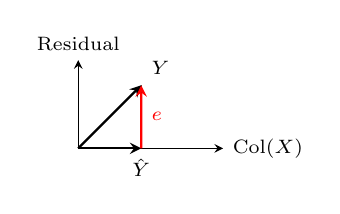
\begin{tikzpicture}[>=stealth,scale=0.8]
    \draw[->] (0,0) -- (2.3,0) node[right] {{\scriptsize Col\( (\vect{X}) \)}};
    \draw[->] (0,0) -- (0,1.4) node[above] {{\scriptsize Residual}};
    \coordinate (Y) at (1, 1);
    \draw[->, thick] (0,0) -- (Y) node[above right] {{\scriptsize \( \vect{Y} \)}};
    \draw[dashed] (Y) -- (1,0);
    \draw[->, thick] (0,0) -- (1,0) node[below] {{\scriptsize \( \hat{\vect{Y}} \)}};
    \draw[->, thick, red] (1,0) -- (Y) node[midway,right] {{\scriptsize \( e \)}};
  \end{tikzpicture}\\[0em]
  \textit{Gauss--Markov theorem:} \( \hat{\beta} \) is the best linear unbiased estimator (minimal variance).
  If \( \varepsilon \) is normal, then \( \hat{\beta} \sim N(\beta,\;\sigma^2(\vect{X}^T \vect{X})^{-1}). \)
  \[ \hat{\vect{Y}} = H \vect{Y} \sim N(\vect{X}\beta,\;\sigma^2 H), \quad  e = (I-H)\vect{Y} \sim N(0,\;\sigma^2 (I-H)). \]
  Moreover, \( \hat{\vect{Y}} \) and \( e \) are independent (since \( H(I-H)=0 \)).\\[0em]
  If an \textit{intercept} (\( \beta_0 \)) is included,
  \begin{align}
    \mathrm{SST}               & = \sum \overbrace{ (\hat{\vect{Y}}_i - \bar{\vect{Y}})^2}^{\mathrm{SSR}} + \sum \overbrace{(\vect{Y}_i-\hat{\vect{Y}}_i)^2}^{\mathrm{SSE}} = \sum (\vect{Y}_i - \bar{\vect{Y}})^2 \\
    \mathrm{SSE}               & = \sum (\vect{Y}_i - \hat{\vect{Y}}_i)^2 = (n - p)\hat{\sigma}^2, \quad \mathrm{SSR} = \sum (\hat{\vect{Y}}_i - \bar{\vect{Y}})^2 = (p-1)\hat{\sigma}^2                           \\
    \mathrm{SST}               & = (n-1)\hat{\sigma}^2, \quad \mathrm{SST} = \mathrm{SSR} + \mathrm{SSE}, \quad \mathrm{SST} = \vect{Y}^T\vect{Y} - n\bar{\vect{Y}}^2                                              \\
    \mathrm{R}^2               & = \dfrac{\mathrm{SSR}}{\mathrm{SST}} = 1 - \dfrac{\mathrm{SSE}}{\mathrm{SST}}, \quad \mathrm{R_{adj}^2} = 1 - \tfrac{n-1}{n-p}\left(1-\mathrm{R^2}\right)                         \\
    \mathrm{df}_{\mathrm{SSR}} & =p-1, \quad \mathrm{df}_{\mathrm{SSE}} = n - p, \quad \mathrm{df}_{\mathrm{SST}}=n-1 \tag{DoF}
  \end{align}
  Under normal errors, \( \mathrm{SSE}/\sigma^2 \sim \chi^2_{\,n-p}\) then \(\mathrm{SSE}\) is independent of \( \hat{\beta} \).
  An unbiased estimator of \( \sigma^2 \) is \( \hat{\sigma}^2 = \tfrac{1}{n-p}\mathrm{SSE}.\)
  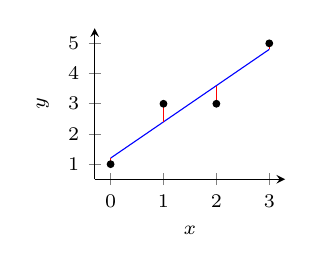
\begin{tikzpicture}
    \begin{axis}[width=4cm, height=3.5cm, xlabel={\( \vect{x} \)}, ylabel={\( \vect{y} \)},
        xlabel style={font=\scriptsize}, ylabel style={font=\scriptsize},
        tick label style={font=\scriptsize},
        xmin=-0.3, xmax=3.3, ymin=0.5, ymax=5.5,
        axis lines=left, xtick={0,1,2,3}, ytick={1,2,3,4,5}]

      % Regression line
      \addplot[domain=0:3, color=blue] {1.2 + 1.2*x};

      % Data points
      \addplot[only marks, mark=*,mark size=1.2] coordinates {(0,1) (1,3) (2,3) (3,5)};

      % Residuals
      \addplot[dashed, color=red] coordinates {(0,1) (0,1.2)};
      \addplot[color=red] coordinates {(1,2.4) (1,3)};
      \addplot[color=red] coordinates {(2,3) (2,3.6)};
      \addplot[color=red] coordinates {(3,4.8) (3,5)};

    \end{axis}
  \end{tikzpicture}
  \section{Inference in Linear Model:}
  For each parameter \( \beta_j \), under \( H_0:\beta_j=0 \),
  \[ t = \frac{\hat{\beta}_j}{\mathrm{SE}(\hat{\beta}_j)} \sim t_{\,n-p}\,.\]
  Thus \((1-\alpha) \) CI for \( \beta_j \) is:
  \[\hat{\beta}_j \pm t_{\,n-p,\;\alpha/2}\; \SE(\hat{\beta}_j) \]
  For a new predictor value \( x_0 \), the predicted response \( \hat{\vect{y}}_0 = x_0 \hat{\beta} \) has \( \mathrm{Var}(\hat{\vect{y}}_0) = \sigma^2\,x_0 (\vect{X}^T \vect{X})^{-1} x_0^T. \)
  A \( (1-\alpha) \) CI for the mean at \( x_0 \) is \( \hat{\vect{y}}_0 \pm t_{\,n-p,\;\alpha/2}\; \hat{\sigma}\,\sqrt{x_0 (\vect{X}^T \vect{X})^{-1} x_0^T}, \)
  and a prediction interval for a new \( \vect{Y} \) at \( x_0 \) is \( \hat{\vect{y}}_0 \pm t_{\,n-p,\;\alpha/2}\; \hat{\sigma}\,\sqrt{x_0 (\vect{X}^T \vect{X})^{-1} x_0^T + 1}\,.  \)

  \section{Hypothesis Testing:}
  \subsection{F-test:}
  For general linear hypothesis \( H_0: L\beta=0 \) where \( L \) is a \( d \times p \) matrix of rank \( d \):
  \[ F = \frac{(L\hat{\beta})^T [L(\vect{X}^T \vect{X})^{-1}L^T]^{-1}(L\hat{\beta})}{\hat{\sigma}^2} \sim F_{d,n-p} \]

  \begin{itemize}[left=0pt,labelsep=1pt,itemsep=0pt]
    \item Testing \( H_0: \beta_j=0 \): \( t^2 = F_{1,n-p} \)
    \item Global test \( H_0: \beta_1=\cdots=\beta_{p-1}=0 \): \( F = \frac{\text{SSR}/(p-1)}{\text{SSE}/(n-p)} \sim F_{p-1,n-p} \)
  \end{itemize}
  If \( F > F_{d,n-p,\alpha} \), reject \( H_0 \) at level \( \alpha \).

  \section{Model Selection:}
  Common criteria: \( \text{AIC} = n\ln(\mathrm{SSE}/n) + 2p, \) \quad
  \( \text{BIC} = n\ln(\mathrm{SSE}/n) + p\ln n \) \quad (smaller is better).
  Mallows' \( C_p \approx \frac{\mathrm{SSE}_{\text{model}}}{\hat{\sigma}^2_{\text{(full)}}} - (n - 2p), \) targeting \( C_p \approx p. \)

  \section{Diagnostics:}
  Residual standard deviation: \( \hat{\sigma} = \sqrt{\mathrm{SSE}/(n-p)}. \)
  Check residual plots for constant variance (no patterns in residuals vs fitted) and for normality (e.g. Q--Q plot).
  High-leverage points: \( h_{ii} = H_{ii} \); large \( h_{ii} \) (relative to \( p/n \)) indicates an outlier in predictor space.
  Standardized residual \( r_i = \frac{e_i}{\hat{\sigma}\sqrt{\,1-h_{ii}\,}} \) (should be \( \approx N(0,1) \) under the model).
  Outliers may have \( |r_i| > 2 \) or \( 3 \).
  Influence can be assessed by Cook's distance: \( D_i = \frac{e_i^2}{p\,\hat{\sigma}^2}\,\frac{h_{ii}}{(1-h_{ii})^2} \) (values \( D_i > 1 \) are often considered large).
  If assumptions are violated (nonlinearity, heteroscedasticity, non-normal errors), consider remedies such as transforming variables or using a different model.
  For variance stabilization, choose \( g(\vect{y}) \) such that \( \mathrm{Var}(g(\vect{Y})) \) is roughly constant.
  E.g. for Poisson \( \vect{Y} \) (Var~\( \vect{\mu} \)), use \( g(\vect{Y})=\sqrt{\vect{Y}} \); for Binomial proportion (\( \mathrm{Var}\approx \vect{\mu}(1-\vect{\mu}) \)), use \( g(\vect{Y})=\arcsin\sqrt{\vect{Y}} \); for \( \mathrm{Var}\propto \vect{\mu}^2 \), use \( \log \vect{Y} \) (Box–Cox power transform can find an optimal \( \lambda \)).

  \section{Multiple Testing:}
  When performing \( m \) hypothesis tests, the family-wise error rate (FWER) at level \( \alpha \) is \( \Pr(\text{any false rejection})\le \alpha. \)\\[0em]
  \textit{Bonferroni correction:} \( \alpha = \frac{\alpha}{m} \) for each test (controls FWER \( \le \alpha \)).\\[0em]
  \textit{S̆idák correction:} \( \alpha = 1 - (1-\alpha)^{1/m} \).\\[0em]
  If \(p_i \le \alpha\) for \(i=1,\dots,m\), reject \(H_0\) for all \(i\) with \(p_i \le \alpha/m\) (Bonferroni) or \(p_i \le 1-(1-\alpha)^{1/m}\) (S̆idák).\\[0em]

  \section{Variance--Stabilising Transformations: Step-by-Step Guide}
  Given a random variable $Y$ with mean $\mu=\mathbb{E}[Y]$ and variance $\mathrm{Var}(Y)=v(\mu)$, a variance–stabilising transformation $g$ is obtained as follows:
  \begin{align}
    \mu                          & = \mathbb{E}[Y], \quad v(\mu) = \mathrm{Var}(Y) \\
    \mathrm{Var}\bigl[g(Y)\bigr] & \approx \bigl[g'(\mu)\bigr]^2 \,v(\mu) = C      \\
    g'(\mu)                      & = \frac{\sqrt{C}}{\sqrt{v(\mu)}}                \\
    g(y)                         & = \sqrt{C}\,\int \frac{dy}{\sqrt{v(y)}}
  \end{align}

  \section{ANOVA (Analysis of Variance):}
  One-way ANOVA with \( a \) groups (levels) and total \( N \) observations: model \( Y_{ij} = \vect{\mu} + \tau_i + \varepsilon_{ij}, \) for \( i=1,\dots,a \) and \( j=1,\dots,n_i, \) where \( \tau_i \) is the effect of group \( i \) (with \( \sum_i \tau_i=0 \)) and \( \varepsilon_{ij}\sim N(0,\sigma^2). \)
  Null hypothesis \( H_0: \tau_1=\tau_2=\cdots=\tau_a=0 \) (all group means equal) is tested by
  \[ F = \frac{\mathrm{SSB}/(a-1)}{\mathrm{SSW}/(N-a)} \sim F_{\,a-1,\,N-a}\,, \]
  where \( \mathrm{SSB}=\sum_{i=1}^a n_i (\bar{\vect{Y}}_i - \bar{\vect{Y}})^2 \) (between-group SS) and \( \mathrm{SSW}=\sum_{i=1}^a\sum_{j=1}^{n_i}(Y_{ij}-\bar{\vect{Y}}_i)^2 \) (within-group SS).
  Total \( \mathrm{SST}=\mathrm{SSB}+\mathrm{SSW} \) with df \( N-1=(a-1)+(N-a). \)
  If \( H_0 \) is rejected, follow-up with multiple-comparison tests (adjusting for multiple testing).
  Two-way ANOVA (two factors) and factorial designs partition variability into main effects and interaction effects similarly, each tested with an F-ratio of mean squares.

  \section{Design of Experiments (DOE):}
  In a \( 2^k \) full factorial design, \( k \) factors each have 2 levels (often coded \( -1 \) and \( +1 \)). All \( 2^k \) combinations are run (possibly with replication). The \textit{main effect} of factor \( A \) is the difference in average response between high and low levels of \( A \); an \textit{interaction} effect (e.g. \( A\!B \)) is the difference in \( A \)'s effect between the two levels of \( B \).
  For example, \( A \) effect \( = \bar{\vect{Y}}(A^+) - \bar{\vect{Y}}(A^-) \), and \( AB \) interaction \( = [(\bar{\vect{Y}}_{A^+B^+}-\bar{\vect{Y}}_{A^-B^+}) - (\bar{\vect{Y}}_{A^+B^-}-\bar{\vect{Y}}_{A^-B^-})] \).
  Effects can be estimated via a regression model \( \vect{Y} = \beta_0 + \sum \beta_i x_i + \sum \beta_{ij}x_i x_j + \cdots \) with \( x_i=\pm1 \). (In this coding, \( \beta_i \) equals half the main effect for factor \( i \), etc.)
  Orthogonal designs: in a full factorial, the design matrix columns for each effect are orthogonal, simplifying estimation and interpretation (no confounding among effects).
  Blocking: to account for nuisance variables, experiments may be divided into blocks. In a \( 2^k \) design with 2 blocks, one effect (usually a high-order interaction) is \textit{confounded} with the block factor (indistinguishable from a block effect).
  E.g. in a \( 2^3 \) design, to run in 2 blocks we can confound the \( ABC \) interaction with blocks by assigning all runs with \( ABC=+1 \) to Block 1 and \( ABC=-1 \) to Block 2. Then any systematic block difference will appear as an \( ABC \) effect (and vice versa).
  Fractional factorial \( 2^{k-p} \) designs run a fraction of the \( 2^k \) runs. Specified by \( p \) \textit{generators} (defining relations).
  E.g. a \( 2^{3-1} \) half-fraction with generator \( I=ABC \) means we run only combinations where \( ABC=+1 \). This yields aliasing: \( A \) is aliased with \( BC \), \( B \) with \( AC \), \( C \) with \( AB \). (Defining relation \( I=ABC \); resolution III design since smallest alias involves 3 factors.)
  Design resolution \( R \): no effect involving \( <R \) factors is aliased with any other effect with \( <R \) factors. Higher resolution designs reduce confounding (e.g. resolution IV: no main effect aliased with any other main or 2-factor effect; resolution V: no main or 2-factor aliased with any other up to 2-factor effect, etc.).
  To de-alias key effects, one can run fold-over (the complementary fraction) or combine fractional designs to a higher resolution.
\end{multicols}

\begin{center}
  \begin{tabular}{|l|l|l|}
    \hline
    \textbf{Metric}            & \textbf{Desired Value} & \textbf{Indicates}           \\
    \hline
    F-statistic                & Large, $p<0.05$        & Model is significant overall \\
    $R^2$                      & High (e.g.\ $>0.7$)    & High variance explained      \\
    Adj.\ $R^2$                & Close to $R^2$         & Efficient use of predictors  \\
    RSE                        & Small                  & Low prediction error         \\
    SE of $\hat\beta_j$        & Small                  & Precise estimates            \\
    $p$-value of $\hat\beta_j$ & $<0.05$                & Significant predictor        \\
    Residuals vs Fitted        & No pattern             & Linearity, homoscedasticity  \\
    QQ-plot                    & Along 45° line         & Normal residuals             \\
    Normality test             & $p>0.05$               & Assumption holds             \\
    \hline
  \end{tabular}
\end{center}

\begin{center}
  \begin{tabular}{l l l}
    \toprule
    \textbf{Ops.}  & \textbf{Rule}                                                                     & \textbf{Cond.}                     \\\midrule
    Indep. $\perp$ & $X\perp Y \Rightarrow \E[XY]=\E[X]\E[Y], \Cov(X,Y)=0$                             & converse only under normality      \\
    Exp. lin.      & $\E[aX+bY+c]=a\E[X]+b\E[Y]+c$                                                     & always                             \\
    Exp. scale     & $\E[aX+b]=a\E[X]+b$                                                               & constants $a,b$ only               \\
    Exp. sum       & $\E[X+Y]=\E[X]+\E[Y]$                                                             & any $X,Y$                          \\
    Exp. prod.     & $\E[XY]=\E[X]\E[Y]$ if $X \perp Y$                                                & independence only                  \\
    Exp. prod. 2   & $\E[XY]=\Cov(X,Y)+\E[X]\E[Y]$ if $X \not\perp Y$                                  & rearranged definition              \\
    Exp. const.    & $\E[c]=c$                                                                         & constant $c$                       \\
    Exp. q. form   & $\E[X^2]=\Var(X)+\E[X]^2$                                                         & any $X$                            \\
    Exp. q. form 2 & $\E[Q]=\E[X^T A X]=\E[X]^T A \E[X] + \mathrm{tr}(A \overbrace{\Var(X)}^{\Sigma})$ & $A$ symmetric, $X$ random vector   \\
    Exp. of var.   & $\E[\Var(X)]=\Var(X)+\E[X]^2$                                                     & any $X$                            \\
    Var. scale     & $\Var(aX+b)=a^{2}\Var(X)$                                                         & shift $b$ does not affect variance \\
    Var. sum       & $\Var(X+Y)=\Var(X)+\Var(Y)+2\Cov(X,Y)$                                            & any $X,Y$                          \\
    Cov. Lin       & $\Cov(X+Y,Z)=\Cov(X,Z)+\Cov(Y,Z)$                                                 & always                             \\
    Cov. scale     & $\Cov(aX+b,\,cY+d)=ac\,\Cov(X,Y)$                                                 & constants $a,c$ only               \\
    Symm.          & $\Cov(X,Y)=\Cov(Y,X)$                                                             & definition                         \\
    Cov--Var link  & $\Cov(X,X)=\Var(X)$                                                               & special case                       \\
    $0$-Cov        & $\Cov(X,Y)=0 \Rightarrow \Var(X\!\pm\!Y)=\Var(X)+\Var(Y)$                         & uncorrelated                       \\
    Matrix form    & $\Cov(A X,\,B Y)=A\,\Cov(X,Y)\,B^{\mathsf T}$                                     & $A,B$ deterministic matrices       \\
    Var. lin. map  & $\Var(A X)=A\,\Var(X)\,A^{\mathsf T}$                                             & take $B=A$ above                   \\
    Exp. prod.     & $\E[XY]=\Cov(X,Y)+\E[X]\E[Y]$                                                     & rearranged definition              \\
    \bottomrule
  \end{tabular}
\end{center}

\begin{center}
  \textbf{NOTATION TABLE}
\end{center}
\begin{center}
  \scriptsize
  \begin{tabular}{l l l}
    \toprule
    \textbf{Symbol}            & \textbf{Meaning}               & \textbf{Interpretation}                                 \\
    \midrule
    \multicolumn{3}{c}{\textbf{Basic Probability \& Statistics}}                                                          \\
    $X, Y, Z$                  & Random variables               & Observable quantities with uncertainty                  \\
    $\vect{X}, \vect{Y}$       & Random vectors                 & Multivariate random quantities                          \\
    $x, y, z$                  & Realizations/observations      & Actual observed values                                  \\
    $\E[X]$                    & Expectation of $X$             & Average/mean value of $X$                               \\
    $\Var(X)$                  & Variance of $X$                & Spread/variability of $X$ around its mean               \\
    $\Cov(X,Y)$                & Covariance                     & How $X$ and $Y$ vary together                           \\
    $\Corr(X,Y)$               & Correlation                    & Standardized covariance, $\in [-1,1]$                   \\
    $X \perp Y$                & Independence                   & $X$ and $Y$ don't influence each other                  \\
    $X \sim N(\mu, \sigma^2)$  & Normal distribution            & $X$ follows normal with mean $\mu$, variance $\sigma^2$ \\
    $\chi^2_k$                 & Chi-squared, $k$ df            & Sum of $k$ squared standard normals                     \\
    $t_k$                      & Student's $t$, $k$ df          & Ratio of normal to chi-squared                          \\
    $F_{d_1,d_2}$              & $F$-distribution               & Ratio of two chi-squared variables                      \\
    \midrule
    \multicolumn{3}{c}{\textbf{Matrix \& Vector Notation}}                                                                \\
    $A, B, \Sigma$             & Matrices                       & Rectangular arrays of numbers                           \\
    $A^T$                      & Transpose                      & Rows become columns                                     \\
    $A^{-1}$                   & Inverse                        & $AA^{-1} = I$ (identity matrix)                         \\
    $|A|, \det(A)$             & Determinant                    & Scaling factor, invertibility measure                   \\
    $\text{tr}(A)$             & Trace                          & Sum of diagonal elements                                \\
    $\text{rank}(A)$           & Rank                           & Number of linearly independent rows/columns             \\
    $I_n$                      & Identity matrix                & $n \times n$ matrix with 1s on diagonal, 0s elsewhere   \\
    $\vect{0}$                 & Zero vector                    & Vector of all zeros                                     \\
    $H^2 = H$                  & Idempotent matrix              & Projection matrix property                              \\
    \midrule
    \multicolumn{3}{c}{\textbf{Linear Regression}}                                                                        \\
    $\vect{Y}$                 & Response vector                & $n \times 1$ vector of outcomes                         \\
    $\vect{X}$                 & Design matrix                  & $n \times p$ matrix of predictors                       \\
    $\beta$                    & Parameter vector               & $p \times 1$ vector of regression coefficients          \\
    $\varepsilon$              & Error vector                   & $n \times 1$ vector of random errors                    \\
    $\hat{\beta}$              & Estimated parameters           & OLS estimate of $\beta$                                 \\
    $\hat{\vect{Y}}$           & Fitted values                  & Predicted responses                                     \\
    $e$                        & Residuals                      & Observed - fitted values                                \\
    $H$                        & Hat matrix                     & Projects onto column space of $\vect{X}$                \\
    $I - H$                    & Residual projection            & Projects onto orthogonal complement                     \\
    $\hat{\sigma}^2$           & Error variance estimate        & Unbiased estimate of $\sigma^2$                         \\
    \midrule
    \multicolumn{3}{c}{\textbf{Sums of Squares}}                                                                          \\
    $\text{SST}$               & Total sum of squares           & Total variation in $\vect{Y}$                           \\
    $\text{SSR}$               & Regression sum of squares      & Variation explained by model                            \\
    $\text{SSE}$               & Error sum of squares           & Unexplained variation                                   \\
    $R^2$                      & Coefficient of determination   & Proportion of variance explained                        \\
    $R_{\text{adj}}^2$         & Adjusted $R^2$                 & $R^2$ penalized for number of parameters                \\
    \midrule
    \multicolumn{3}{c}{\textbf{Hypothesis Testing}}                                                                       \\
    $H_0$                      & Null hypothesis                & Statement being tested                                  \\
    $H_1$                      & Alternative hypothesis         & What we believe if $H_0$ is false                       \\
    $\alpha$                   & Significance level             & Probability of Type I error                             \\
    $p$-value                  & Probability value              & Evidence against $H_0$                                  \\
    $t$                        & $t$-statistic                  & Test statistic for single parameters                    \\
    $F$                        & $F$-statistic                  & Test statistic for multiple parameters                  \\
    $\text{df}$                & Degrees of freedom             & Parameters available for estimation                     \\
    \midrule
    \multicolumn{3}{c}{\textbf{Model Diagnostics}}                                                                        \\
    $h_{ii}$                   & Leverage                       & Influence of observation $i$ on its own fit             \\
    $r_i$                      & Standardized residual          & Residual scaled by its standard error                   \\
    $D_i$                      & Cook's distance                & Overall influence of observation $i$                    \\
    $\text{SE}(\hat{\beta}_j)$ & Standard error                 & Uncertainty in parameter estimate                       \\
    \midrule
    \multicolumn{3}{c}{\textbf{ANOVA}}                                                                                    \\
    $\tau_i$                   & Treatment effect               & Effect of $i$-th group/treatment                        \\
    $\text{SSB}$               & Between-group SS               & Variation between group means                           \\
    $\text{SSW}$               & Within-group SS                & Variation within groups                                 \\
    $a$                        & Number of groups               & Groups/treatments in the experiment                     \\
    $N$                        & Total observations             & Total sample size across all groups                     \\
    \midrule
    \multicolumn{3}{c}{\textbf{Model Selection}}                                                                          \\
    $\text{AIC}$               & Akaike Information Criterion   & Balances fit and complexity                             \\
    $\text{BIC}$               & Bayesian Information Criterion & More conservative than AIC                              \\
    $C_p$                      & Mallows' $C_p$                 & Measures prediction error                               \\
    \midrule
    \multicolumn{3}{c}{\textbf{Design of Experiments}}                                                                    \\
    $2^k$                      & Full factorial                 & All combinations of $k$ factors at 2 levels             \\
    $2^{k-p}$                  & Fractional factorial           & Subset of full factorial                                \\
    $A^+, A^-$                 & Factor levels                  & High and low levels of factor $A$                       \\
    $AB$                       & Interaction effect             & Combined effect of factors $A$ and $B$                  \\
    \bottomrule
  \end{tabular}
\end{center}

\begin{center}
  \textbf{KEY FORMULAS \& WHAT THEY TELL US}
\end{center}
\begin{center}
  \scriptsize
  \begin{tabular}{l p{8cm}}
    \toprule
    \textbf{Formula}                                                            & \textbf{What It Tells Us}                                               \\
    \midrule
    $\hat{\beta} = (\vect{X}^T\vect{X})^{-1}\vect{X}^T\vect{Y}$                 & Best linear unbiased estimator minimizing squared errors                \\
    $\text{Var}(\hat{\beta}) = \sigma^2(\vect{X}^T\vect{X})^{-1}$               & Uncertainty in parameter estimates depends on error variance and design \\
    $t = \frac{\hat{\beta}_j}{\text{SE}(\hat{\beta}_j)}$                        & How many standard errors the estimate is from zero                      \\
    $F = \frac{\text{MS}_{\text{model}}}{\text{MS}_{\text{error}}}$             & Ratio of explained to unexplained variation                             \\
    $R^2 = \frac{\text{SSR}}{\text{SST}}$                                       & Fraction of total variation explained by the model                      \\
    $(\vect{X} - \vect{\mu})^T\Sigma^{-1}(\vect{X} - \vect{\mu}) \sim \chi^2_p$ & Mahalanobis distance measures how far from center                       \\
    $H = \vect{X}(\vect{X}^T\vect{X})^{-1}\vect{X}^T$                           & Projects data onto the space spanned by predictors                      \\
    $\text{SST} = \text{SSR} + \text{SSE}$                                      & Total variation splits into explained and unexplained parts             \\
    $\text{AIC} = n\ln(\text{SSE}/n) + 2p$                                      & Balance between goodness of fit and model complexity                    \\
    $D_i = \frac{e_i^2}{p\hat{\sigma}^2} \cdot \frac{h_{ii}}{(1-h_{ii})^2}$     & Measures how much fitted values change when observation $i$ is removed  \\
    \bottomrule
  \end{tabular}
\end{center}
\end{document}
